\documentclass{article}

\usepackage[english]{babel}
\usepackage[utf8]{inputenc}
\usepackage{amsmath}
\usepackage{graphicx}
\graphicspath{ {./images/} }
\usepackage{color}
\usepackage{textcomp}
\usepackage{etoolbox}    
\usepackage{listings}
\newcount\mymark
\makeatletter
\def\mycoderef#1{%
  \global\advance\mymark by 1%
  \protected@write \@auxout {}{\string \newlabel {#1}{{\the\mymark}{}}}%
  \makebox[0pt][r]{{\scriptsize\bfseries \the\mymark~}}%
}
%%% Taken from https://www.entwickler-ecke.de/topic_C+Darstellung+fuer+Latex+listings_100839,0.html

\usepackage{color}
\usepackage{listings}    
\usepackage{courier}


%%% Define Custom IDE Colors %%%
\definecolor{arduinoGreen}    {rgb} {0.17, 0.43, 0.01}
\definecolor{arduinoGrey}     {rgb} {0.47, 0.47, 0.33}
\definecolor{arduinoOrange}   {rgb} {0.8 , 0.4 , 0   }
\definecolor{arduinoBlue}     {rgb} {0.01, 0.61, 0.98}
\definecolor{arduinoDarkBlue} {rgb} {0.0 , 0.2 , 0.5 }

%%% Define Arduino Language %%%
\lstdefinelanguage{Arduino}{
  language=C++, % begin with default C++ settings 
%
%
  %%% Keyword Color Group 1 %%%  (called KEYWORD3 by arduino)
  keywordstyle=\color{arduinoGreen},   
  deletekeywords={  % remove all arduino keywords that might be in c++
break, case, override, final, continue, default, do, else, for, if, return, goto, switch, throw, try, while, setup, loop, export, not, or, and, xor, include, define, elif, else, error, if, ifdef, ifndef, pragma, warning,HIGH, LOW, INPUT, INPUT_PULLUP, OUTPUT, DEC, BIN, HEX, OCT, PI, HALF_PI, TWO_PI, LSBFIRST, MSBFIRST, CHANGE, FALLING, RISING, DEFAULT, EXTERNAL, INTERNAL, INTERNAL1V1, INTERNAL2V56, LED_BUILTIN, LED_BUILTIN_RX, LED_BUILTIN_TX, DIGITAL_MESSAGE, FIRMATA_STRING, ANALOG_MESSAGE, REPORT_DIGITAL, REPORT_ANALOG, SET_PIN_MODE, SYSTEM_RESET, SYSEX_START, auto, int8_t, int16_t, int32_t, int64_t, uint8_t, uint16_t, uint32_t, uint64_t, char16_t, char32_t, operator, enum, delete, bool, boolean, byte, char, const, false, float, double, null, NULL, int, long, new, private, protected, public, short, signed, static, volatile, String, void, true, unsigned, word, array, sizeof, dynamic_cast, typedef, const_cast, struct, static_cast, union, friend, extern, class, reinterpret_cast, register, explicit, inline, _Bool, complex, _Complex, _Imaginary, atomic_bool, atomic_char, atomic_schar, atomic_uchar, atomic_short, atomic_ushort, atomic_int, atomic_uint, atomic_long, atomic_ulong, atomic_llong, atomic_ullong, virtual, PROGMEM, Serial, Serial1, Serial2, Serial3, SerialUSB, Keyboard, Mouse,abs, acos, asin, atan, atan2, ceil, constrain, cos, degrees, exp, floor, log, map, max, min, radians, random, randomSeed, round, sin, sq, sqrt, tan, pow, bitRead, bitWrite, bitSet, bitClear, bit, highByte, lowByte, analogReference, analogRead, 
analogReadResolution, analogWrite, analogWriteResolution, 
attachInterrupt, detachInterrupt, digitalPinToInterrupt, delay, delayMicroseconds, digitalWrite, digitalRead, interrupts, millis, micros, noInterrupts, noTone, pinMode, pulseIn, pulseInLong, shiftIn, shiftOut, tone, yield, Stream, begin, end, peek, read, print, println, available, availableForWrite, flush, setTimeout, find, findUntil, parseInt, parseFloat, readBytes, readBytesUntil, readString, readStringUntil, trim, toUpperCase, toLowerCase, charAt, compareTo, concat, endsWith, startsWith, equals, equalsIgnoreCase, getBytes, indexOf, lastIndexOf, length, replace, setCharAt, substring, toCharArray, toInt, press, release, releaseAll, accept, click, move, isPressed, isAlphaNumeric, isAlpha, isAscii, isWhitespace, isControl, isDigit, isGraph, isLowerCase, isPrintable, isPunct, isSpace, isUpperCase, isHexadecimalDigit, 
                }, morekeywords={   % add arduino structures to group 1\\
  break, case, override, final, continue, default, do, else, for, if, return, goto, switch, throw, try, while, setup, loop, export, not, or, and, xor, include, define, elif, else, error, if, ifdef, ifndef, pragma, warning,}, 
% 
%
  %%% Keyword Color Group 2 %%%  (called LITERAL1 by arduino)
  keywordstyle=[2]\color{arduinoBlue},   
  keywords=[2]{   % add variables and dataTypes as 2nd group  
HIGH, LOW, INPUT, INPUT_PULLUP, OUTPUT, DEC, BIN, HEX, OCT, PI, HALF_PI, TWO_PI, LSBFIRST, MSBFIRST, CHANGE, FALLING, RISING, DEFAULT, EXTERNAL, INTERNAL, INTERNAL1V1, INTERNAL2V56, LED_BUILTIN, LED_BUILTIN_RX, LED_BUILTIN_TX, DIGITAL_MESSAGE, FIRMATA_STRING, ANALOG_MESSAGE, REPORT_DIGITAL, REPORT_ANALOG, SET_PIN_MODE, SYSTEM_RESET, SYSEX_START, auto, int8_t, int16_t, int32_t, int64_t, uint8_t, uint16_t, uint32_t, uint64_t, char16_t, char32_t, operator, enum, delete, bool, boolean, byte, char, const, false, float, double, null, NULL, int, long, new, private, protected, public, short, signed, static, volatile, String, void, true, unsigned, word, array, sizeof, dynamic_cast, typedef, const_cast, struct, static_cast, union, friend, extern, class, reinterpret_cast, register, explicit, inline, _Bool, complex, _Complex, _Imaginary, atomic_bool, atomic_char, atomic_schar, atomic_uchar, atomic_short, atomic_ushort, atomic_int, atomic_uint, atomic_long, atomic_ulong, atomic_llong, atomic_ullong, virtual, PROGMEM,},  
% 
%
  %%% Keyword Color Group 3 %%%  (called KEYWORD1 by arduino)
  keywordstyle=[3]\bfseries\color{arduinoOrange},
  keywords=[3]{  % add built-in functions as a 3rd group
                Serial, Serial1, Serial2, Serial3, SerialUSB, Keyboard, Mouse,
                },      
%
%
  %%% Keyword Color Group 4 %%%  (called KEYWORD2 by arduino)
  keywordstyle=[4]\color{arduinoOrange},
  keywords=[4]{  % add more built-in functions as a 4th group
abs, acos, asin, atan, atan2, ceil, constrain, cos, degrees, exp, floor, log, map, max, min, radians, random, randomSeed, round, sin, sq, sqrt, tan, pow, bitRead, bitWrite, bitSet, bitClear, bit, highByte, lowByte, analogReference, analogRead, 
analogReadResolution, analogWrite, analogWriteResolution, 
attachInterrupt, detachInterrupt, digitalPinToInterrupt, delay, delayMicroseconds, digitalWrite, digitalRead, interrupts, millis, micros, noInterrupts, noTone, pinMode, pulseIn, pulseInLong, shiftIn, shiftOut, tone, yield, Stream, begin, end, peek, read, print, println, available, availableForWrite, flush, setTimeout, find, findUntil, parseInt, parseFloat, readBytes, readBytesUntil, readString, readStringUntil, trim, toUpperCase, toLowerCase, charAt, compareTo, concat, endsWith, startsWith, equals, equalsIgnoreCase, getBytes, indexOf, lastIndexOf, length, replace, setCharAt, substring, toCharArray, toInt, press, release, releaseAll, accept, click, move, isPressed, isAlphaNumeric, isAlpha, isAscii, isWhitespace, isControl, isDigit, isGraph, isLowerCase, isPrintable, isPunct,isSpace, isUpperCase, isHexadecimalDigit,},      
%
%
  %%% Set Other Colors %%%
  stringstyle=\color{arduinoDarkBlue},    
  commentstyle=\color{arduinoGrey},    
%          
%   
  %%%% Line Numbering %%%%
   numbers=left,                    
  numbersep=5pt,                   
  numberstyle=\color{arduinoGrey},    
  %stepnumber=2,                      % show every 2 line numbers
%
%
  %%%% Code Box Style %%%%
  breaklines=true,                    % wordwrapping
  tabsize=2,         
  basicstyle=\ttfamily  
}

\begin{document}

\begin{titlepage}
\pagenumbering{gobble}
\addcontentsline{toc}{section}{Abstract}
\begin{center}
\vspace{1cm}
\huge
\textbf{My E-Gardener}

\LARGE
\vspace{.5cm}
IT-project with regard to our B.Sc in Software Engineering at the University of The Faroe Islands


\vspace{.5cm}
\textbf{Kristmund Ryggstein and Hergeir Winther Lognberg}\\
\vspace{.5cm}
\Large
\vspace{.5cm}
\vfill
\begin{center}
Faculty of Science and Technology

Benadikt Joensen, Gunnar Restorff

University of the Faroe Islands

January 2019

\pagebreak
\Large
\textbf{Abstract}

\end{center}
We were asked to do an it project using an Arduino Uno. We chose to to do an automated gardening system with it, because that is relevent for some work projects that are currently in progress on Sandoy, where we are from. Our ardunio project entails an automated system that waters, measures moisture, heat and light exposure. That is done by customizing an Arduino Uno which has a moisture-, heat and light sensor that does all our measurements. All the the data is then collected by the Arduino, and then sent to a Web Service via. a esp-05 wifi module. The Web Service receives the data, and presents it to the user. The user is registered with the Web Service, and can track his plant data through his registered user account, where he also can customize water input for the plant/s.


\end{center}
\end{titlepage}
\pagenumbering{gobble}
\tableofcontents
\listoffigures
\listoftables
\pagebreak
\pagenumbering{gobble}
\begin{center}\section*{Acknowledgments}\end{center}
\addcontentsline{toc}{section}{Acknowledgments}

\pagebreak
\pagenumbering{arabic}
\section{Introduction}

We have chosen to work with automatic a gardening system because it has some tasks, what we believe, are tedious and easy to forget. There has been an increasing interest on Sandoy in trying to grow more vegetables on the islands, and to sell them. That grown interest in thanks to initiatives such as "Veltan" and "Eplafestivalurin". Trying to be self-sufficient with regards to food produce is, according us, a good idea, and that's were we think that our modest electronic gardening project fits well with that philosophy, and will be an interest for those, who want to try to be more self-sufficient.
 
\section{Setup}
The Arduino Uno, TMP36GZ heat sensor, resistors and the cables which we use in this project, was provided by the one responsible by the course. We used at the start a FC28 moisture sensor, but it generally uses DC current which means that it corrodes quickly because of electrolysis in the soil and alters the soil composition which could potentially damage the plant, which would eventually lead to tainted readings. We changed it to use an AC pulse that can be seen in figure, but we decided to opt for Capacitive Soil Moisture Sensor V1.2 that is Corrosion Resistant. The FC28 sensor can be seen in figure 1.

\subsection{FC28}

Our intention was to use the Arduino to induce an alternating current through the sensor. To simplify things, we circumvented the circuit of FC-28 such that we connected directly to the pins on the sensor. To alternate the current, we first emit 5V from pin 12 and set pin 13 to low (0V) for 1 ms then we take a reading through the analog pin A0. Then we flip the pin 12 and 13 ( 5V from pin 13 ) for the same amount of time. This should somewhat remedy the problems of electrolysis by shifting the ions back and forth between the moisture sensor pins, instead of just letting them congest at one pin. The chip had to be removed so that it could use AC.
The setup can be seen above.
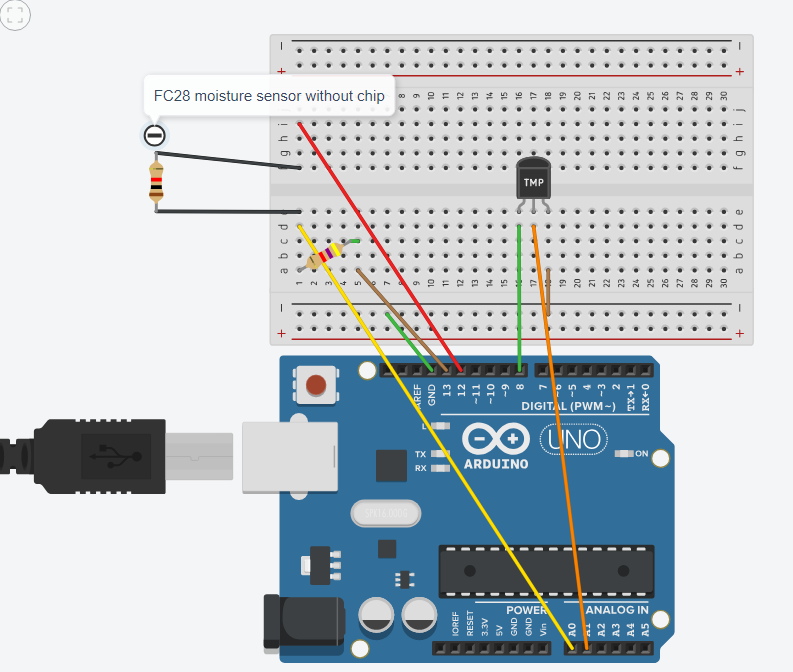
\includegraphics[scale = 0.50]{FC-28-Diagram.PNG}


The resistor in the circuit helps increase the amount of current entering the analog sensor. Without it about half the current would go in the pin 13 when the measurement occurs. We are therefor able to steer the range of current entering the analog input. The left left leg is connected to 8 digital pin, the middle leg is connected to A1 pin, and the third leg is connected to -18 on the breadboard which is then connected to the ground pin on the Arduino.  


\subsection{TMP Sensor}

The TMP36 temperature is fairly simple. It can measure degrees from -50\textdegree{}C to \textdegree{250}C, where it has a precision of 0.1\textdegree{}C\footnote{https://www.bc-robotics.com/tutorials/using-a-tmp36-temperature-sensor-with-arduino/}. It works as a diode so when it changes temperature, it then its voltage changes accordingly. The sensor measures the small change and outputs an analog output based on it, so its possible to calculate the temperature according to that output. We use a readCelcius() method from the Temperature Class, and it can be seen below.
\pagebreak
\begin{lstlisting}[language=Arduino]
const int8_t TemperatureSensor::readCelsius()
{
    digitalWrite(triggerPin, HIGH);
    delayMicroseconds(200);
    uint16_t reading = analogRead(readPin);
    digitalWrite(triggerPin, LOW);
    // converting that reading to voltage, for 3.3v arduino use 3.3
    double voltage = reading * 5.0; // * 0.0009775171;
    voltage /= 1024.0;
    return round((voltage - 0.5) * 100);
}

\end{lstlisting}

reading = analogRead(readPind) reads the output from the sensor, then it's converted to voltage by multiplying with five. That is then divided by 1024 to find the percentage of the analog read, because the arduino outputs between 0 and 1023, where 0 is not voltage and 1023 is 5V. Five is then subtracted from that, and then that result is multiplied with 100 to convert it ffrom mV to degrees. Five is subtracted from the reading, because we want it so that 0V corresponds to -50\textdegree{}C
\pagebreak

\section{Attachments}
\begin{figure}
  \centering
      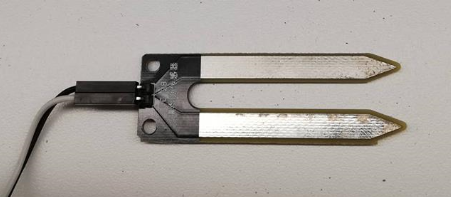
\includegraphics{fc-28-corrosion}
  \caption{Corroded fc-28 after moderate use.}
\end{figure}


\pagebreak
\pagenumbering{gobble}
\addcontentsline{toc}{section}{References}
\bibliographystyle{ieeetr}
\nocite{*}
% \bibliography{biblio.bib}
% change the file name to line up with your bibtex file


\end{document}